% !TEX root = ../main.tex
% !TEX program = xelatex
\section{问题四的模型建立与求解}

\subsection{求解思路}

问题四在问题二、三的基础上引入\textbf{实时波动电价}。每天制定购电计划时，不仅未来负载和光伏未知，未来电价也不能提前获得。若仍按固定电价安排储能，可能在并不便宜的时段提前充电，或在高价时段到来前过早放电。因此，需要先判断未来电价，再与供需预测和电池状态一起确定购电安排。

问题四包含两种运行方式。问题四-2每天0:00确定当天订单，日内不能修改，供需预测和储能运行沿用问题二。问题四-3则沿用问题三的近期加权负载预测、日内负载校正和光伏融合方法，并在6:00、12:00和18:00调整尚未执行的订单。两条分支分别保留原有的信息条件与调整权限。

电价预测考虑历史同刻中位数、岭回归和提升树三种方法。同刻中位数能够保留常见的日内价格形状，但较难反映近期供需变化。提升树可以描述价格与多种因素之间的非线性关系，适合零点缺少当天观测的情况。日内已有实际价格作为参照，岭回归能够用较清楚的线性关系修正判断，并限制相关特征造成的系数波动。据此，问题四-2采用\textbf{提升树预测与零点规划}，问题四-3采用\textbf{岭回归预测与日内滚动规划}，并通过实际费用比较检验这一选择。

\subsection{波动电价预测}

历史电价具有较稳定的日内规律和周重复特征，但同一时刻在不同日期仍有变化。预测输入包括附件1的日内电价、最近四周同星期同刻的价格中位数、最近7天同刻中位数、上周同刻价格，以及星期、季节位置和预测净负载。同星期历史不足时，改用近期同刻价格。日内再将当天已发生价格减去历史同刻基准，取差值中位数表示当天整体偏高或偏低的程度，并加入最后一个已结束时段的偏差。为区分短时波动与持续变化，还分别加入按6小时、1小时时间尺度指数衰减的偏差特征；这些当天偏差只用于当天剩余时段，零点时取零。

其中，净负载由各分支自己的负载预测减去光伏预测得到。历史训练样本也按当时能够获得的信息构造，实际价格只有发生后才能作为训练目标或日内反馈。

\subsubsection*{（1）问题四-2：提升树价格预测}

每天0:00尚未获得当天实际价格，主要依靠历史价格和供需背景进行预测。采用直方图梯度提升树，将多棵较小的回归树逐步相加：

\begin{equation}
\hat{p}
=
F_0(\mathbf{x})
+
\gamma
\sum_{m=1}^{M}
h_m(\mathbf{x}),
\end{equation}

其中，$\mathbf{x}$为上述价格特征，$F_0$为初始预测，$h_m$用于修正此前预测的残差。取$M=100$、学习率$\gamma=0.05$，每棵树最多包含31个叶节点。较小的学习率使每棵树只作有限修正，避免一次过度追随历史波动。

\subsubsection*{（2）问题四-3：岭回归价格预测}

在6:00、12:00和18:00，可以利用当天已经发生的实际价格。历史同刻价格与近期价格往往较为接近，直接回归容易让它们的系数相互抵消并过度放大。岭回归在拟合误差之外加入系数惩罚，使价格判断更加平稳：

\begin{equation}
\min_{\beta_0,\boldsymbol{\beta}}
\sum_i
\left(
p_i-\beta_0-\mathbf{z}_i^{\mathrm T}\boldsymbol{\beta}
\right)^2
+
\lambda_p
\sum_j\beta_j^2,
\qquad
\lambda_p=10.
\end{equation}

其中，$p_i$为训练样本的实际电价，$\mathbf{z}_i$为标准化后的特征，$\beta_0$和$\boldsymbol{\beta}$分别为截距与回归系数。标准化所需的均值和标准差仅由当前训练窗口计算。各特征标准化后，设置正则系数$\lambda_p=10$，对过大的回归系数施加惩罚，以限制相关价格特征之间的系数抵消和放大。该设置下，岭回归在候选比较中以接近最低的费用获得较少的紧急购电，因而用于日内分支。预测时使用
\begin{equation}
\hat p_{t|\tau}=\max\left\{0.001,\,\beta_0+\mathbf{z}_{t|\tau}^{\mathrm T}\boldsymbol{\beta}\right\},
\end{equation}
其中$\tau$沿用问题三的决策时点记号，$t$为待预测时段。下限用于避免回归外推产生非正电价；提升树及历史参照的预测也统一保留这一正下限。

两类价格模型均每7天训练一次，使用最近56天已经发生的数据；历史不足56天时使用已有样本。日内各时点更新模型输入和预测结果，无需每天重新拟合四次模型。

\subsection{波动电价下的购电模型}

\subsubsection*{（1）问题四-2}

问题四-2直接沿用问题二的负载、光伏预测、误差准备和储能约束，将固定电价替换为0:00预测得到的波动电价。目标函数为

\begin{equation}
\min J_{4-2}
=
\sum_{t\in T_0}
\hat{p}_{t|0}q_t
-
\nu S_T,
\end{equation}

其中，$T_0$为零点开始的规划时段，$q_t$为普通购电量，$S_T$为规划末端储电量，$\nu$沿用前文的末端电量参考价值。

规划延伸至次日24:00，以避免模型在当天末尾过早放空电池，但只固定当天订单。实际运行中，普通购电和电池放电仍无法满足的缺口，按照该时段\textbf{实际电价的5倍}紧急补购。

\subsubsection*{（2）问题四-3}

问题四-3将问题三的供需预测与本问的价格预测共同代入滚动规划。零点根据近期加权的同星期负载和光伏预报制定订单；6:00、12:00和18:00利用已发生负载、新光伏预报与已发生价格更新后续判断。误差准备仍由这些供需预测自身的历史误差计算。

设零点原计划为$q_t^0$，调整后的订单为$q_t$，则目标函数为

\begin{equation}
\min J_{4-3}
=
\sum_{t\in \mathcal T_{\tau}}
\hat{p}_{t|\tau}
\left(q_t+5e_t\right)
+
\frac{1}{2}
\sum_{t\in \mathcal A_{\tau}}
\hat{p}_{t|\tau}
\left|q_t-q_t^0\right|
-
\nu S_T,
\end{equation}

其中，$e_t$为预计紧急购电量，$\mathcal T_{\tau}$为当前时点至次日24:00的规划时段，
$\mathcal A_{\tau}$为当天尚未执行且已在零点订电的时段。
零点决策时$\mathcal A_0$为空，次日辅助订单也不收调整费。
第一项衡量购电费用，第二项衡量改变零点订单的代价，末项保留电池对后续用电的价值。

已经执行的订单不再修改。同一时段经过多次调整时，只按最终订单与零点原计划之间的净变化结算一次。规划使用预测电价；最终普通购电费、调整费和紧急购电费均按对应执行时段的实际电价结算。

供需平衡、储电递推、$1200$--$10800\ \mathrm{kWh}$容量限制、$5000\ \mathrm{kW}$充放电功率限制及各$90\%$的充放电效率均沿用前文。实际日末储电量继续传递至次日，不再要求每日首尾相等。

\subsection{模型求解与方案选择}

给定供需预测和价格预测后，两条分支均为线性规划，采用HiGHS求解。各策略均从第6.5节的共同库存8592.69 kWh出发，按时间顺序模拟2025年2月1日至12月31日的334天。每次决策读取真实当前储电量，求得订单后执行至下一决策时点，再更新供需与储电状态。

为比较价格模型，在各分支内固定供需预测、设备参数和初始储电量，只改变价格预测方法，结果见表\ref{tab:q4_price_comparison}。

\begin{table}[H]
    \centering
    \caption{波动电价下不同价格预测模型的比较}
    \label{tab:q4_price_comparison}
    \begin{tabular}{ccccc}
        \hline
        分支 & 价格模型 & 价格MAE/(元/kWh) & 总费用/万元 & 紧急购电量/kWh \\
        \hline
        问题四-2 & 历史同刻中位数 & 0.04984 & 1427.22 & 97728.89 \\
        问题四-2 & 岭回归 & 0.04472 & 1426.64 & 99205.19 \\
        问题四-2 & 提升树 & \textbf{0.03884} & \textbf{1425.52} & 98725.98 \\
        \hline
        问题四-3 & 历史同刻中位数 & 0.04676 & 1383.78 & 40144.52 \\
        问题四-3 & 岭回归 & 0.04442 & 1382.29 & \textbf{38733.80} \\
        问题四-3 & 提升树 & \textbf{0.03834} & \textbf{1382.06} & 40116.12 \\
        \hline
    \end{tabular}
    \par\smallskip
    \begin{minipage}{0.96\textwidth}
    \small 注：价格模型比较固定采用四周同星期等权负载，不作日内负载校正；表中提升树均为15叶。该表用于比较价格预测方法，完整策略的费用另见表\ref{tab:q4_final_results}。
    \end{minipage}
\end{table}

问题四-2中，提升树的预测误差和购电费用均最低，说明非线性价格预测适合零点制定整日订单的条件。其叶节点数再由下文的复杂度检验确定。

问题四-3中，提升树的预测误差更小，但在上述相同供需条件下，其费用仅比岭回归低约0.016\%，紧急购电量却更多。可见，价格预测误差更小并不一定带来更合适的储能安排。综合费用、紧急补购和解释难度，本文采用岭回归，将其与问题三的负载校正及滚动调整结构结合。

\subsection{结果与分析}

两种策略的全年费用见表\ref{tab:q4_final_results}。其中，问题四-2采用31叶提升树；问题四-3采用岭回归，误差准备取0.60分位。

\begin{table}[H]
    \centering
    \caption{问题四两种策略的全年费用结果}
    \label{tab:q4_final_results}
    \begin{tabular}{lrr}
        \hline
        指标 & 问题四-2 & 问题四-3 \\
        \hline
        普通购电费/元 & 13613522.32 & 13212221.00 \\
        调整费/元 & 0.00 & 299775.47 \\
        紧急购电费/元 & 635048.55 & 183933.22 \\
        \textbf{总费用/元} & \textbf{14248570.87} & \textbf{13695929.70} \\
        紧急购电量/kWh & 98756.33 & 32162.76 \\
        \hline
    \end{tabular}
\par\smallskip
{\small 注：各项分别保留两位小数，合计由未舍入费用计算。}
\end{table}

问题四-3的总费用为1369.59万元，比问题四-2减少55.26万元，约下降3.88\%。虽然日内改约产生了调整费，但普通购电和紧急补购的费用下降更多。及时修正供需与价格判断，使后续订单更接近实际需要，也让电池有机会重新安排充放电。

55.26万元的节省来自供需判断、价格预测和订单调整的共同改进，体现了日内信息更新与滚动调度的综合价值。波动电价也不只是改变账单上的单价：它会改变提前购电是否合算，进而影响日末储电量和后续日期的运行。

四个指定日期的结果见表\ref{tab:q4_specified_dates}。普通订单、紧急补购和日末余电共同反映各日实际安排，费用包含普通购电、调整及紧急购电。
% Generated from saved trajectories by scripts/restore_review_tables.py.
\begin{table}[H]
\centering
\caption{问题四两条分支的指定日期结果}
\label{tab:q4_specified_dates}
\small
\setlength{\tabcolsep}{5pt}
\begin{tabular}{llrrrr}
\toprule
分支 & 日期 & 普通订单/kWh & 紧急购电/kWh & 日末储电/kWh & 总费用/元 \\
\midrule
四-2 & 3月20日 & 62329.63 & 329.13 & 1376.30 & 41909.16 \\
四-2 & 6月21日 & 42375.21 & 0.00 & 10380.22 & 20358.11 \\
四-2 & 9月23日 & 68066.93 & 10.23 & 2592.35 & 44700.97 \\
四-2 & 12月21日 & 94612.77 & 0.00 & 9798.14 & 71357.71 \\
\midrule
四-3 & 3月20日 & 61627.63 & 16.86 & 1386.88 & 40429.92 \\
四-3 & 6月21日 & 42677.14 & 0.00 & 10800.00 & 20343.61 \\
四-3 & 9月23日 & 66331.89 & 247.01 & 2815.47 & 45166.06 \\
四-3 & 12月21日 & 93273.34 & 51.32 & 8176.08 & 72209.10 \\
\bottomrule
\end{tabular}
\par\smallskip
\begin{minipage}{0.96\textwidth}
\small 注：普通订单为全天最终订单之和；总费用按实际电价计算，包含普通购电、调整与紧急购电。
\end{minipage}
\end{table}

指定日期的费用差异随当天预测偏差和储电状态而变化：日内方案在3月20日费用较低，在9月23日和12月21日费用较高。考虑储电量跨日衔接，本文以完整评价期总费用衡量整体效果，日内方案累计节省55.26万元。

\subsection{模型检验}

利用实际供需逐10分钟复核供需平衡、储电递推、容量与功率限制，并按真实电价重新计算费用。
储电轨迹和费用均与计算结果一致，差异处于浮点误差范围内。
模型训练和日内预测均以当前时点为数据截止，保证购电安排只依据当时已知的信息。

在此基础上，分别检查问题四-2的树复杂度和问题四-3的准备程度。前者影响价格预测的细致程度，后者直接决定多订普通电与承担紧急补购之间的取舍，结果如图\ref{fig:q4_model_test}所示。

\begin{figure}[H]
    \centering
    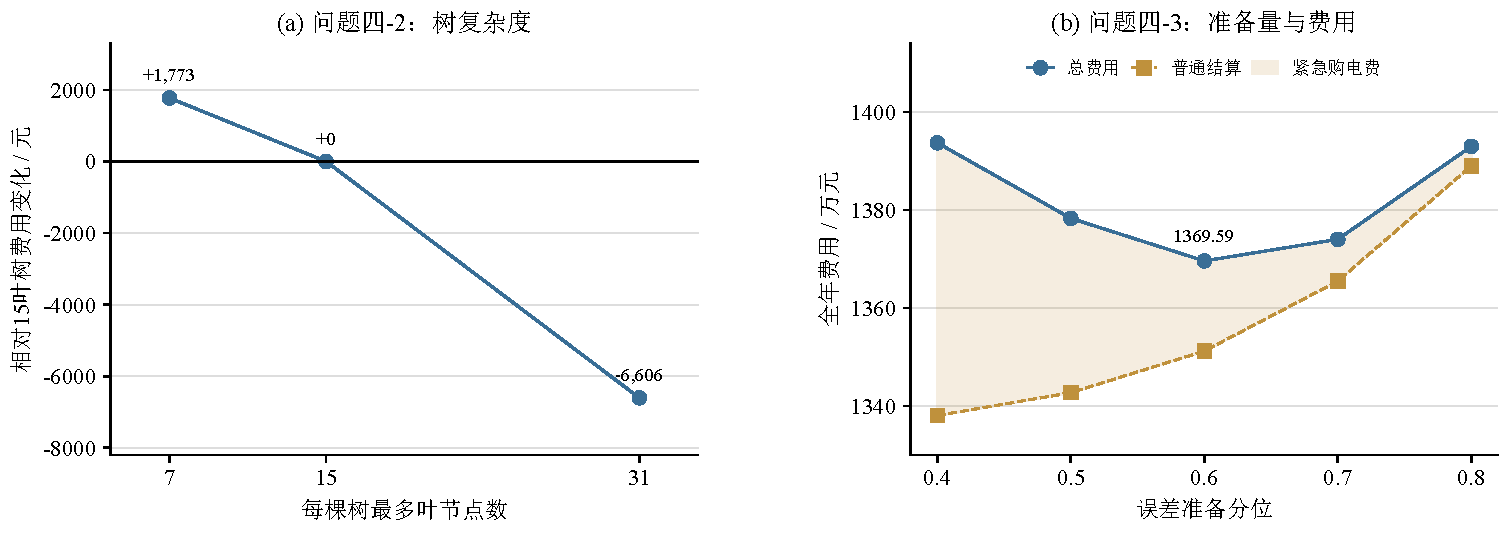
\includegraphics[width=0.95\textwidth]{fig/q4_final_validation.pdf}
    \caption{树复杂度与误差准备的费用检验}
    \label{fig:q4_model_test}
\end{figure}

\subsubsection*{（1）提升树复杂度检验}

图\ref{fig:q4_model_test}(a)以15叶模型为参照。7叶模型费用略有增加，31叶模型减少约6606元，说明适当增加叶节点有助于刻画更细的价格差异。进一步按实际电价的5\%、50\%、95\%分位对期末可放电量估值，31叶模型仍比15叶模型节省5890.24--6423.72元，费用排序保持一致。因此，选择31叶模型有实际费用依据，其优势也不依赖于少留期末电量。

\subsubsection*{（2）误差准备与补购风险}

图\ref{fig:q4_model_test}(b)比较0.40至0.80五档准备分位。分位偏低时，普通购电较少，但预测不足容易转化为五倍电价的紧急补购；分位偏高时，紧急费用下降，却增加了普通购电和存不下的订单。总费用在0.60附近最低，因此本问取0.60分位。

0.60分位在普通订电与紧急补购之间取得较好的费用平衡。提高至0.70虽能进一步减少紧急购电，但总费用增加约4.41万元，因此保留0.60。

评价期内发生紧急补购188天，补购电量约3.22万$\mathrm{kWh}$，各时段负载均得到满足。在最高5\%的实际电价区间，紧急补购约1.07万kWh，表明后续风险控制可重点针对高价时段的缺口识别与储能准备。
